\documentclass[tikz]{standalone}
\usepackage{ensps-colorscheme}

\begin{document}
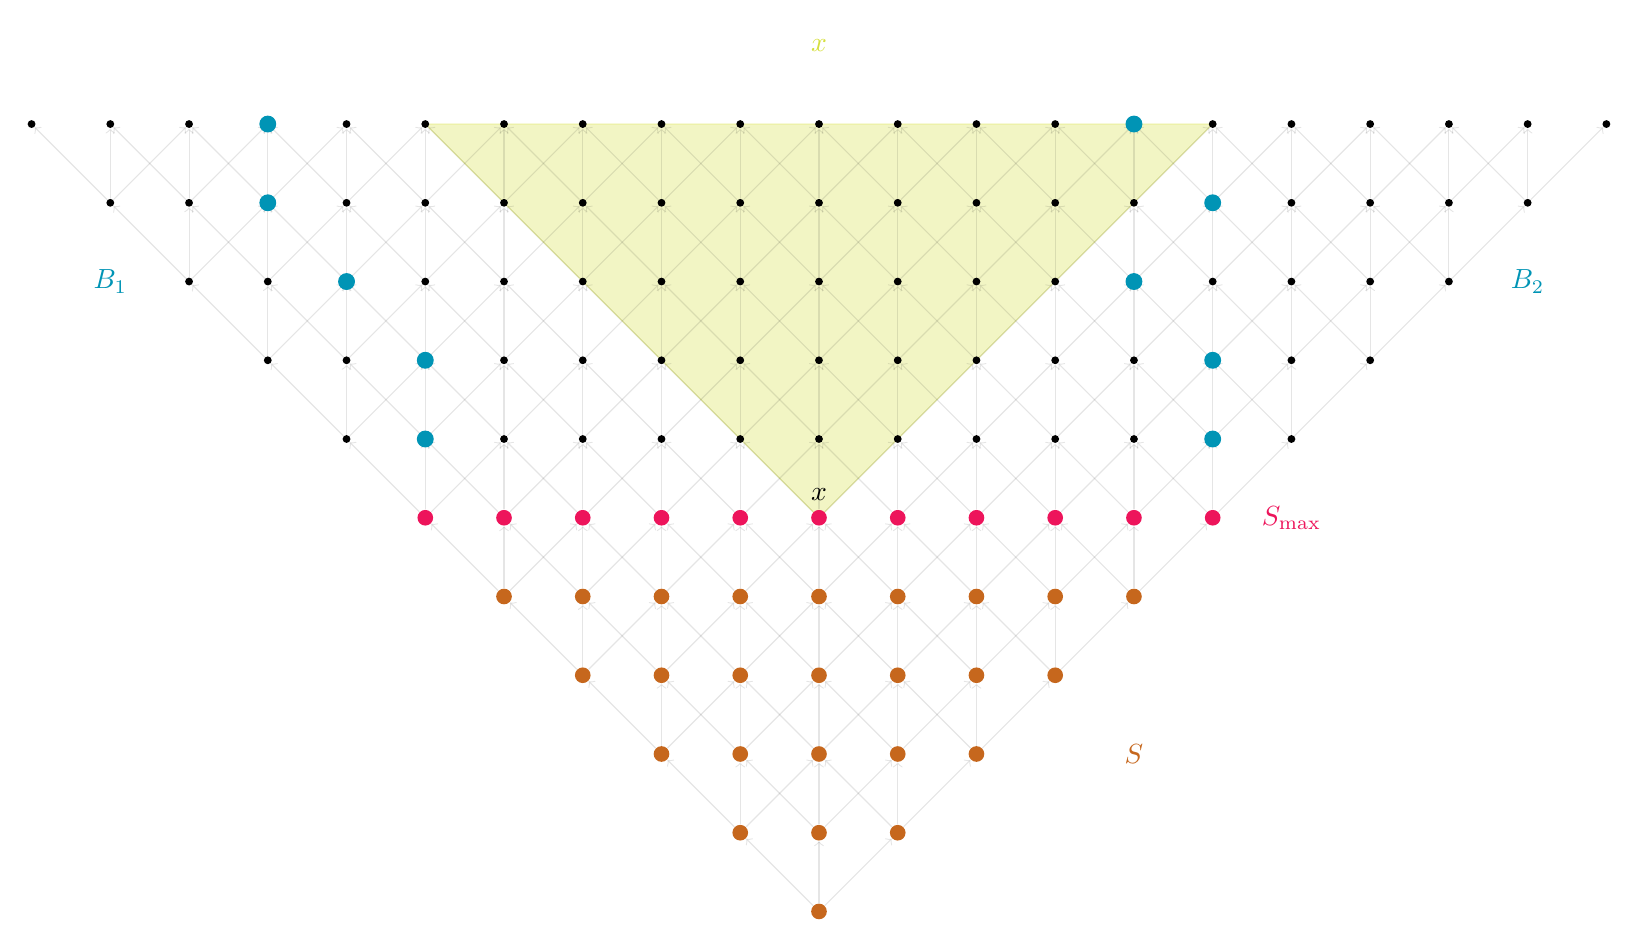
\begin{tikzpicture}[
    every node/.style={
        inner sep=2pt,
        minimum width=1pt,
        circle,
        fill,
    },
    inS/.style={C3},
    notInS/.style={inner sep=1pt},
    inSmax/.style={B2},
    inBranch/.style={fill=C4,C4},
    upclosure/.style={D5,fill=D5,opacity=0.3},
    label/.style={
        fill=none,
        opacity=1,
    },
    ]
    % The picture is quite simple, we just have a triangle
    % of "bottom elements" called $S$
    % and the top edge of this triangle contains points 
    % that have "wires" going out from them (branches)
    % We create a list of points
    \draw[upclosure] (0,5) -- (-5,10) -- (5,10) -- cycle;
    \foreach \level in {0,...,4} {
        \foreach[count=\xi] \item in {-\level, ..., \level} {
            \node[inS] (L\level N\xi) at (\item, \level) {};
        }
    }
    \foreach[count=\xi] \item in {-5, ..., 5} {
        \node[inS,inSmax] (L5N\xi) at (\item, 5) {};
    }
    \foreach \level in {6,...,10} {
        \foreach[count=\xi] \item in {-\level, ..., \level} {
            \node[notInS] (L\level N\xi) at (\item, \level) {};
        }
    }

    \foreach \level in {0,...,9} {
        \pgfmathsetmacro{\levelp}{int(\level + 1)}
        \foreach[count=\xi] \item in {-\level, ..., \level} {
            \pgfmathsetmacro{\yir}{int(\xi + 1)}
            \pgfmathsetmacro{\yil}{int(\xi + 2)}
            \draw[opacity=0.1,->] (L\level N\xi) -- (L\levelp N\yil);
            \draw[opacity=0.1,->] (L\level N\xi) -- (L\levelp N\xi);
            \draw[opacity=0.1,->] (L\level N\xi) -- (L\levelp N\yir);
        }
    }

    \foreach \level/\xi in {6/2,7/3,8/3,9/3,10/4} {
        \draw[inBranch] (L\level N\xi) circle (0.1);
    }
    \foreach \level/\xi in {6/12,7/13,8/13,9/15,10/15} {
        \draw[inBranch] (L\level N\xi) circle (0.1);
    }


    \node[inS,label] (SLabel) at (4,2) {$S$};
    \node[inSmax,label] (SmaxLabel) at (6,5) {$S_{\max}$};
    \node[upclosure,label] (upLabel)   at (0,11) {$\upset{x}$};
    \node[inBranch,label] (b1Label)    at (-9,8) {$B_1$};
    \node[inBranch,label] (b2Label)    at (9,8)  {$B_2$};
    \node[label] (xlabel) at (0,5.3) {$x$};


\end{tikzpicture}
\end{document}
